% mnras_guide.tex
%
% MNRAS LaTeX user guide
%
% v3.0 released 22 May 2015
% (version numbers match those of mnras.cls)
%
% Copyright (C) Royal Astronomical Society 2015
% Authors:
% Keith T. Smith (Royal Astronomical Society)

% Change log
%
% v3.0   September 2013 - May 2015
%    First version: complete rewrite of the user guide
%    Basic structure taken from mnras_template.tex by the same author

%%%%%%%%%%%%%%%%%%%%%%%%%%%%%%%%%%%%%%%%%%%%%%%%%%
% Basic setup. Most papers should leave these options alone.
\documentclass[a4paper,fleqn,usenatbib,useAMS]{mnras}

%%%%% AUTHORS - PLACE YOUR OWN PACKAGES HERE %%%%%

% Only include extra packages if you really need them. Common packages are:
\usepackage{graphicx}	% Including figure files
\usepackage{amsmath}	% Advanced maths commands
\usepackage{amssymb}	% Extra maths symbols
\usepackage{multicol}        % Multi-column entries in tables
\usepackage{bm}		% Bold maths symbols, including upright Greek
\usepackage{pdflscape}	% Landscape pages

%%%%%%%%%%%%%%%%%%%%%%%%%%%%%%%%%%%%%%%%%%%%%%%%%%

%%%%%% AUTHORS - PLACE YOUR OWN MACROS HERE %%%%%%

% Please keep new commands to a minimum, and use \newcommand not \def to avoid
% overwriting existing commands. Example:
%\newcommand{\pcm}{\,cm$^{-2}$}	% per cm-squared
\newcommand{\kms}{\,km\,s$^{-1}$} % kilometres per second
\newcommand{\bibtex}{\textsc{Bib}\!\TeX} % bibtex. Not quite the correct typesetting, but close enough

%%%%%%%%%%%%%%%%%%%%%%%%%%%%%%%%%%%%%%%%%%%%%%%%%%


% Use vector fonts, so it zooms properly in on-screen viewing software
% Don't change these lines unless you know what you are doing
\usepackage[T1]{fontenc}
\usepackage{ae,aecompl}

% MNRAS is set in Times font. If you don't have this installed (most LaTeX
% installations will be fine) or prefer the old Computer Modern fonts, comment
% out the following line
\usepackage{newtxtext,newtxmath}
% Depending on your LaTeX fonts installation, you might get better results with one of these:
%\usepackage{mathptmx}
%\usepackage{txfonts}

%%%%%%%%%%%%%%%%%%% TITLE PAGE %%%%%%%%%%%%%%%%%%%

% Title of the paper, and the short title which is used in the headers.
% Keep the title short and informative.
\title[MNRAS \LaTeX\ guide for authors]{\textit{Monthly Notices of the Royal Astronomical
  Society}: \\ \LaTeX\ guide for authors}

% The list of authors, and the short list which is used in the headers.
% If you need two or more lines of authors, add an extra line using \newauthor
\author[K. T. Smith]{Keith T. Smith$^{1}$\thanks{Contact e-mail: \href{mailto:mn@ras.org.uk}{mn@ras.org.uk}}\thanks{Present address: Science magazine, AAAS Science International, \mbox{82-88}~Hills Road, Cambridge CB2~1LQ, UK}
\\
% List of institutions
$^{1}$Royal Astronomical Society, Burlington House, Piccadilly, London W1J 0BQ, UK}

% These dates will be filled out by the publisher
\date{Last updated 2015 May 22; in original form 2013 September 5}

% Enter the current year, for the copyright statements etc.
\pubyear{2015}

% Don't change these lines
\begin{document}
\label{firstpage}
\pagerange{\pageref{firstpage}--\pageref{lastpage}}
\maketitle

% Abstract of the paper
\begin{abstract}
This is a guide for preparing papers for \textit{Monthly Notices of the Royal Astronomical Society} using the \verb'mnras' \LaTeX\ package.
It provides instructions for using the additional features in the document class.
This is not a general guide on how to use \LaTeX, and nor does it replace the journal's instructions to authors.
See \texttt{mnras\_template.tex} for a simple template.
\end{abstract}

% Select between one and six entries from the list of approved keywords.
% Don't make up new ones.
\begin{keywords}
editorials, notices -- miscellaneous
\end{keywords}

%%%%%%%%%%%%%%%%%%%%%%%%%%%%%%%%%%%%%%%%%%%%%%%%%%

%%%%%%%%%%%%%%%%% BODY OF PAPER %%%%%%%%%%%%%%%%%%

% The MNRAS class isn't designed to include a table of contents, but for this document one is useful.
% I therefore have to do some kludging to make it work without masses of blank space.
\begingroup
\let\clearpage\relax
\tableofcontents
\endgroup
\newpage

\section{Introduction}

The journal \textit{Monthly Notices of the Royal Astronomical Society} (MNRAS) encourages authors to prepare their papers using \LaTeX.
The style file \verb'mnras.cls' can be used to approximate the final appearance of the journal, and provides numerous features to simplify the preparation of papers.
This document, \verb'mnras_guide.tex', provides guidance on using that style file and the features it enables.

This is not a general guide on how to use \LaTeX, of which many excellent examples already exist.
We particularly recommend \textit{Wikibooks \LaTeX}\footnote{\url{https://en.wikibooks.org/wiki/LaTeX}}, a collaborative online textbook which is of use to both beginners and experts.
Alternatively there are several other online resources, and most academic libraries also hold suitable beginner's guides.

For guidance on the contents of papers, journal style, and how to submit a paper, see the MNRAS Instructions to Authors\footnote{\label{foot:itas}\url{http://www.oxfordjournals.org/our_journals/mnras/for_authors/}}.
Only technical issues with the \LaTeX\ class are considered here.


\section{Obtaining and installing the MNRAS package}
Some \LaTeX\ distributions come with the MNRAS package by default.
If yours does not, you can either install it using your distribution's package manager, or download it from the Comprehensive \TeX\ Archive Network\footnote{\url{http://www.ctan.org/tex-archive/macros/latex/contrib/mnras}} (CTAN).

The files can either be installed permanently by placing them in the appropriate directory (consult the documentation for your \LaTeX\ distribution), or used temporarily by placing them in the working directory for your paper.

To use the MNRAS package, simply specify \verb'mnras' as the document class at the start of a \verb'.tex' file:

\begin{verbatim}
\documentclass{mnras}
\end{verbatim}
Then compile \LaTeX\ (and if necessary \bibtex) in the usual way.

\section{Preparing and submitting a paper}
We recommend that you start with a copy of the \texttt{mnras\_template.tex} file.
Rename the file, update the information on the title page, and then work on the text of your paper.
Guidelines for content, style etc. are given in the instructions to authors on the journal's website$^{\ref{foot:itas}}$.
Note that this document does not follow all the aspects of MNRAS journal style (e.g. it has a table of contents).

If a paper is accepted, it is professionally typeset and copyedited by the publishers.
It is therefore likely that minor changes to presentation will occur.
For this reason, we ask authors to ignore minor details such as slightly long lines, extra blank spaces, or misplaced figures, because these details will be dealt with during the production process.

Papers must be submitted electronically via the online submission system; paper submissions are not permitted.
For full guidance on how to submit a paper, see the instructions to authors.

\section{Class options}
\label{sec:options}
There are several options which can be added to the document class line like this:

\begin{verbatim}
\documentclass[option1,option2]{mnras}
\end{verbatim}
The available options are:
\begin{itemize}
\item \verb'letters' -- used for papers in the journal's Letters section.
\item \verb'onecolumn' -- single column, instead of the default two columns. This should be used {\it only} if necessary for the display of numerous very long equations.
\item \verb'doublespacing' -- text has double line spacing. Please don't submit papers in this format.
\item \verb'referee' -- \textit{(deprecated)} single column, double spaced, larger text, bigger margins. Please don't submit papers in this format.
\item \verb'galley' -- \textit{(deprecated)} no running headers, no attempt to align the bottom of columns.
\item \verb'landscape' -- \textit{(deprecated)} sets the whole document on landscape paper.
\item \verb"usenatbib" -- \textit{(all papers should use this)} this uses Patrick Daly's \verb"natbib.sty" package for citations.
\item \verb"usegraphicx" -- \textit{(most papers will need this)} includes the \verb'graphicx' package, for inclusion of figures and images.
\item \verb'useAMS' -- adds support for upright Greek characters \verb'\upi', \verb'\umu' and \verb'\upartial' ($\upi$, $\umu$ and $\upartial$). Only these three are included, if you require other symbols you will need to include the \verb'amsmath' or \verb'amsymb' packages (see section~\ref{sec:packages}).
\item \verb"usedcolumn" -- includes the package \verb"dcolumn", which includes two new types of column alignment for use in tables.
\end{itemize}

Some of these options are deprecated and retained for backwards compatibility only.
Others are used in almost all papers, but again are retained as options to ensure that papers written decades ago will continue to compile without problems.
If you want to include any other packages, see section~\ref{sec:packages}.

\section{Title page}

If you are using \texttt{mnras\_template.tex} the necessary code for generating the title page, headers and footers is already present.
Simply edit the title, author list, institutions, abstract and keywords as described below.

\subsection{Title}
There are two forms of the title: the full version used on the first page, and a short version which is used in the header of other odd-numbered pages (the `running head').
Enter them with \verb'\title[]{}' like this:
\begin{verbatim}
\title[Running head]{Full title of the paper}
\end{verbatim}
The full title can be multiple lines (use \verb'\\' to start a new line) and may be as long as necessary, although we encourage authors to use concise titles. The running head must be $\le~45$ characters on a single line.

See appendix~\ref{sec:advanced} for more complicated examples.

\subsection{Authors and institutions}

Like the title, there are two forms of author list: the full version which appears on the title page, and a short form which appears in the header of the even-numbered pages. Enter them using the \verb'\author[]{}' command.

If the author list is more than one line long, start a new line using \verb'\newauthor'. Use \verb'\\' to start the institution list. Affiliations for each author should be indicated with a superscript number, and correspond to the list of institutions below the author list.

For example, if I were to write a paper with two coauthors at another institution, one of whom also works at a third location:
\begin{verbatim}
\author[K. T. Smith et al.]{
Keith T. Smith,$^{1}$
A. N. Other,$^{2}$
and Third Author$^{2,3}$
\\
$^{1}$Affiliation 1\\
$^{2}$Affiliation 2\\
$^{3}$Affiliation 3}
\end{verbatim}
Affiliations should be in the format `Department, Institution, Street Address, City and Postal Code, Country'.

Email addresses can be inserted with the \verb'\thanks{}' command which adds a title page footnote.
If you want to list more than one email, put them all in the same \verb'\thanks' and use \verb'\footnotemark[]' to refer to the same footnote multiple times.
Present addresses (if different to those where the work was performed) can also be added with a \verb'\thanks' command.

\subsection{Abstract and keywords}

The abstract is entered in an \verb'abstract' environment:
\begin{verbatim}
\begin{abstract}
The abstract of the paper.
\end{abstract}
\end{verbatim}
\noindent Note that there is a word limit on the length of abstracts.
For the current word limit, see the journal instructions to authors$^{\ref{foot:itas}}$.

Immediately following the abstract, a set of keywords is entered in a \verb'keywords' environment:
\begin{verbatim}
\begin{keywords}
keyword 1 -- keyword 2 -- keyword 3
\end{keywords}
\end{verbatim}
\noindent There is a list of permitted keywords, which is agreed between all the major astronomy journals and revised every few years.
Do \emph{not} make up new keywords!
For the current list of allowed keywords, see the journal's instructions to authors$^{\ref{foot:itas}}$.

\section{Sections and lists}

Sections and lists are generally the same as in the standard \LaTeX\ classes.

\subsection{Sections}
\label{sec:sections}
Sections are entered in the usual way, using \verb'\section{}' and its variants. It is possible to nest up to four section levels:
\begin{verbatim}
\section{Main section}
 \subsection{Subsection}
  \subsubsection{Subsubsection}
   \paragraph{Lowest level section}
\end{verbatim}
\noindent The other \LaTeX\ sectioning commands \verb'\part', \verb'\chapter' and \verb'\subparagraph{}' are deprecated and should not be used.

Some sections are not numbered as part of journal style (e.g. the Acknowledgements).
To insert an unnumbered section use the `starred' version of the command: \verb'\section*{}'.

See appendix~\ref{sec:advanced} for more complicated examples.

\subsection{Lists}

Two forms of lists can be used in MNRAS -- numbered and unnumbered.

For a numbered list, use the \verb'enumerate' environment:
\begin{verbatim}
\begin{enumerate}
 \item First item
 \item Second item
 \item etc.
\end{enumerate}
\end{verbatim}
\noindent which produces
\begin{enumerate}
 \item First item
 \item Second item
 \item etc.
\end{enumerate}
Note that the list uses lowercase Roman numerals, rather than the \LaTeX\ default Arabic numerals.

For an unnumbered list, use the \verb'description' environment without the optional argument:
\begin{verbatim}
\begin{description}
 \item First item
 \item Second item
 \item etc.
\end{description}
\end{verbatim}
\noindent which produces
\begin{description}
 \item First item
 \item Second item
 \item etc.
\end{description}

Bulleted lists using the \verb'itemize' environment should not be used in MNRAS; it is retained for backwards compatibility only.

\section{Mathematics and symbols}

The MNRAS class mostly adopts standard \LaTeX\ handling of mathematics, which is briefly summarised here.
See also section~\ref{sec:packages} for packages that support more advanced mathematics.

Mathematics can be inserted into the running text using the syntax \verb'$1+1=2$', which produces $1+1=2$.
Use this only for short expressions or when referring to mathematical quantities; equations should be entered as described below.

\subsection{Equations}
Equations should be entered using the \verb'equation' environment, which automatically numbers them:

\begin{verbatim}
\begin{equation}
 a^2=b^2+c^2
\end{equation}
\end{verbatim}
\noindent which produces
\begin{equation}
 a^2=b^2+c^2
\end{equation}

By default, the equations are numbered sequentially throughout the whole paper. If a paper has a large number of equations, it may be better to number them by section (2.1, 2.2 etc.). To do this, add the command \verb'\numberwithin{equation}{section}' to the preamble.

It is also possible to produce un-numbered equations by using the \LaTeX\ built-in \verb'\['\textellipsis\verb'\]' and \verb'$$'\textellipsis\verb'$$' commands; however MNRAS requires that all equations are numbered, so these commands should be avoided.

\subsection{Special symbols}


\begin{table}
 \caption{Additional commands for special symbols commonly used in astronomy. These can be used anywhere.}
 \label{tab:anysymbols}
 \begin{tabular}{lll}
  \hline
  Command & Output & Meaning\\
  \hline
  \verb'\sun' & \sun & Sun, solar\\[2pt] % additional height spacing for enhanced symbol legibility
  \verb'\earth' & \earth & Earth, terrestrial\\[2pt]
  \verb'\micron' & \micron & microns\\[2pt]
  \verb'\degr' & \degr & degrees\\[2pt]
  \verb'\arcmin' & \arcmin & arcminutes\\[2pt]
  \verb'\arcsec' & \arcsec & arcseconds\\[2pt]
  \verb'\fdg' & \fdg & fraction of a degree\\[2pt]
  \verb'\farcm' & \farcm & fraction of an arcminute\\[2pt]
  \verb'\farcs' & \farcs & fraction of an arcsecond\\[2pt]
  \verb'\fd' & \fd & fraction of a day\\[2pt]
  \verb'\fh' & \fh & fraction of an hour\\[2pt]
  \verb'\fm' & \fm & fraction of a minute\\[2pt]
  \verb'\fs' & \fs & fraction of a second\\[2pt]
  \verb'\fp' & \fp & fraction of a period\\[2pt]
  \verb'\diameter' & \diameter & diameter\\[2pt]
  \verb'\sq' & \sq & square, Q.E.D.\\[2pt]
  \hline
 \end{tabular}
\end{table}

\begin{table}
 \caption{Additional commands for mathematical symbols. These can only be used in maths mode.}
 \label{tab:mathssymbols}
 \begin{tabular}{lll}
  \hline
  Command & Output & Meaning\\
  \hline
  \verb'\upi' & $\upi$ & upright pi\\[2pt] % additional height spacing for enhanced symbol legibility
  \verb'\umu' & $\umu$ & upright mu\\[2pt]
  \verb'\upartial' & $\upartial$ & upright partial derivative\\[2pt]
  \verb'\lid' & $\lid$ & less than or equal to\\[2pt]
  \verb'\gid' & $\gid$ & greater than or equal to\\[2pt]
  \verb'\la' & $\la$ & less than of order\\[2pt]
  \verb'\ga' & $\ga$ & greater than of order\\[2pt]
  \verb'\loa' & $\loa$ & less than approximately\\[2pt]
  \verb'\goa' & $\goa$ & greater than approximately\\[2pt]
  \verb'\cor' & $\cor$ & corresponds to\\[2pt]
  \verb'\sol' & $\sol$ & similar to or less than\\[2pt]
  \verb'\sog' & $\sog$ & similar to or greater than\\[2pt]
  \verb'\lse' & $\lse$ & less than or homotopic to \\[2pt]
  \verb'\gse' & $\gse$ & greater than or homotopic to\\[2pt]
  \verb'\getsto' & $\getsto$ & from over to\\[2pt]
  \verb'\grole' & $\grole$ & greater over less\\[2pt]
  \verb'\leogr' & $\leogr$ & less over greater\\
  \hline
 \end{tabular}
\end{table}

Some additional symbols of common use in astronomy have been added in the MNRAS class. These are shown in tables~\ref{tab:anysymbols}--\ref{tab:mathssymbols}. The command names are -- as far as possible -- the same as those used in other major astronomy journals.

Many other mathematical symbols are also available, either built into \LaTeX\ or via additional packages. If you want to insert a specific symbol but don't know the \LaTeX\ command, we recommend using the Detexify website\footnote{\url{http://detexify.kirelabs.org}}.

Sometimes font or coding limitations mean a symbol may not get smaller when used in sub- or superscripts, and will therefore be displayed at the wrong size. There is no need to worry about this as it will be corrected by the typesetter during production.

To produce bold symbols in mathematics, use \verb'\bmath' for simple variables, and the \verb'bm' package for more complex symbols (see section~\ref{sec:packages}). Vectors are set in bold italic, using \verb'\mathbfit{}'.

For matrices, use \verb'\mathbfss{}' to produce a bold sans-serif font e.g. \mathbfss{H}; this works even outside maths mode, but not all symbols are available (e.g. Greek). For $\nabla$ (del, used in gradients, divergence etc.) use \verb'$\nabla$'.

\subsection{Ions}

A new \verb'\ion{}{}' command has been added to the class file, for the correct typesetting of ionisation states.
For example, to typeset singly ionised calcium use \verb'\ion{Ca}{ii}', which produces \ion{Ca}{ii}.

\section{Figures and tables}
\label{sec:fig_table}
Figures and tables (collectively called `floats') are mostly the same as built into \LaTeX.

\subsection{Basic examples}
\begin{figure}
 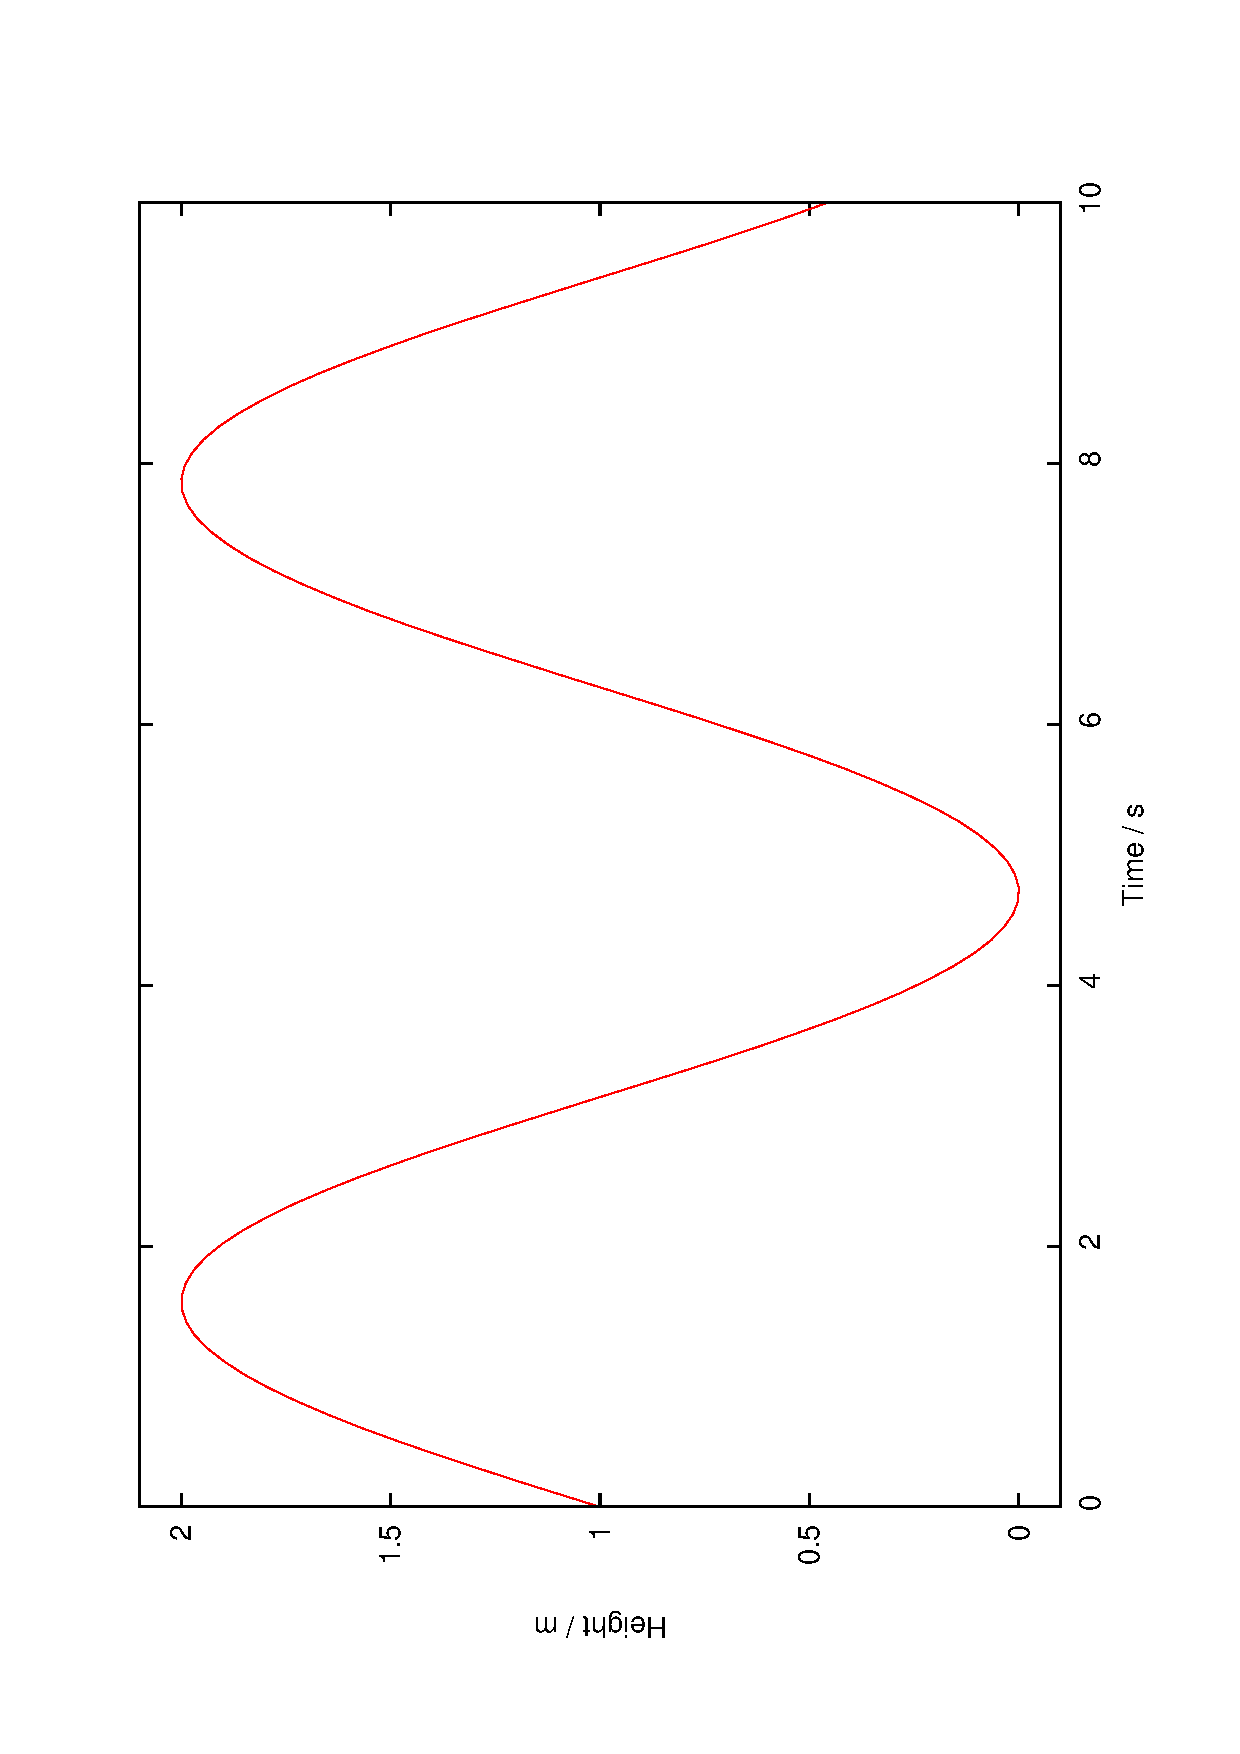
\includegraphics[width=\columnwidth]{example}
 \caption{An example figure.}
 \label{fig:example}
\end{figure}
Figures are inserted in the usual way using a \verb'figure' environment and \verb'\includegraphics'. The example Figure~\ref{fig:example} was generated using the code:
\begin{verbatim}
\begin{figure}
 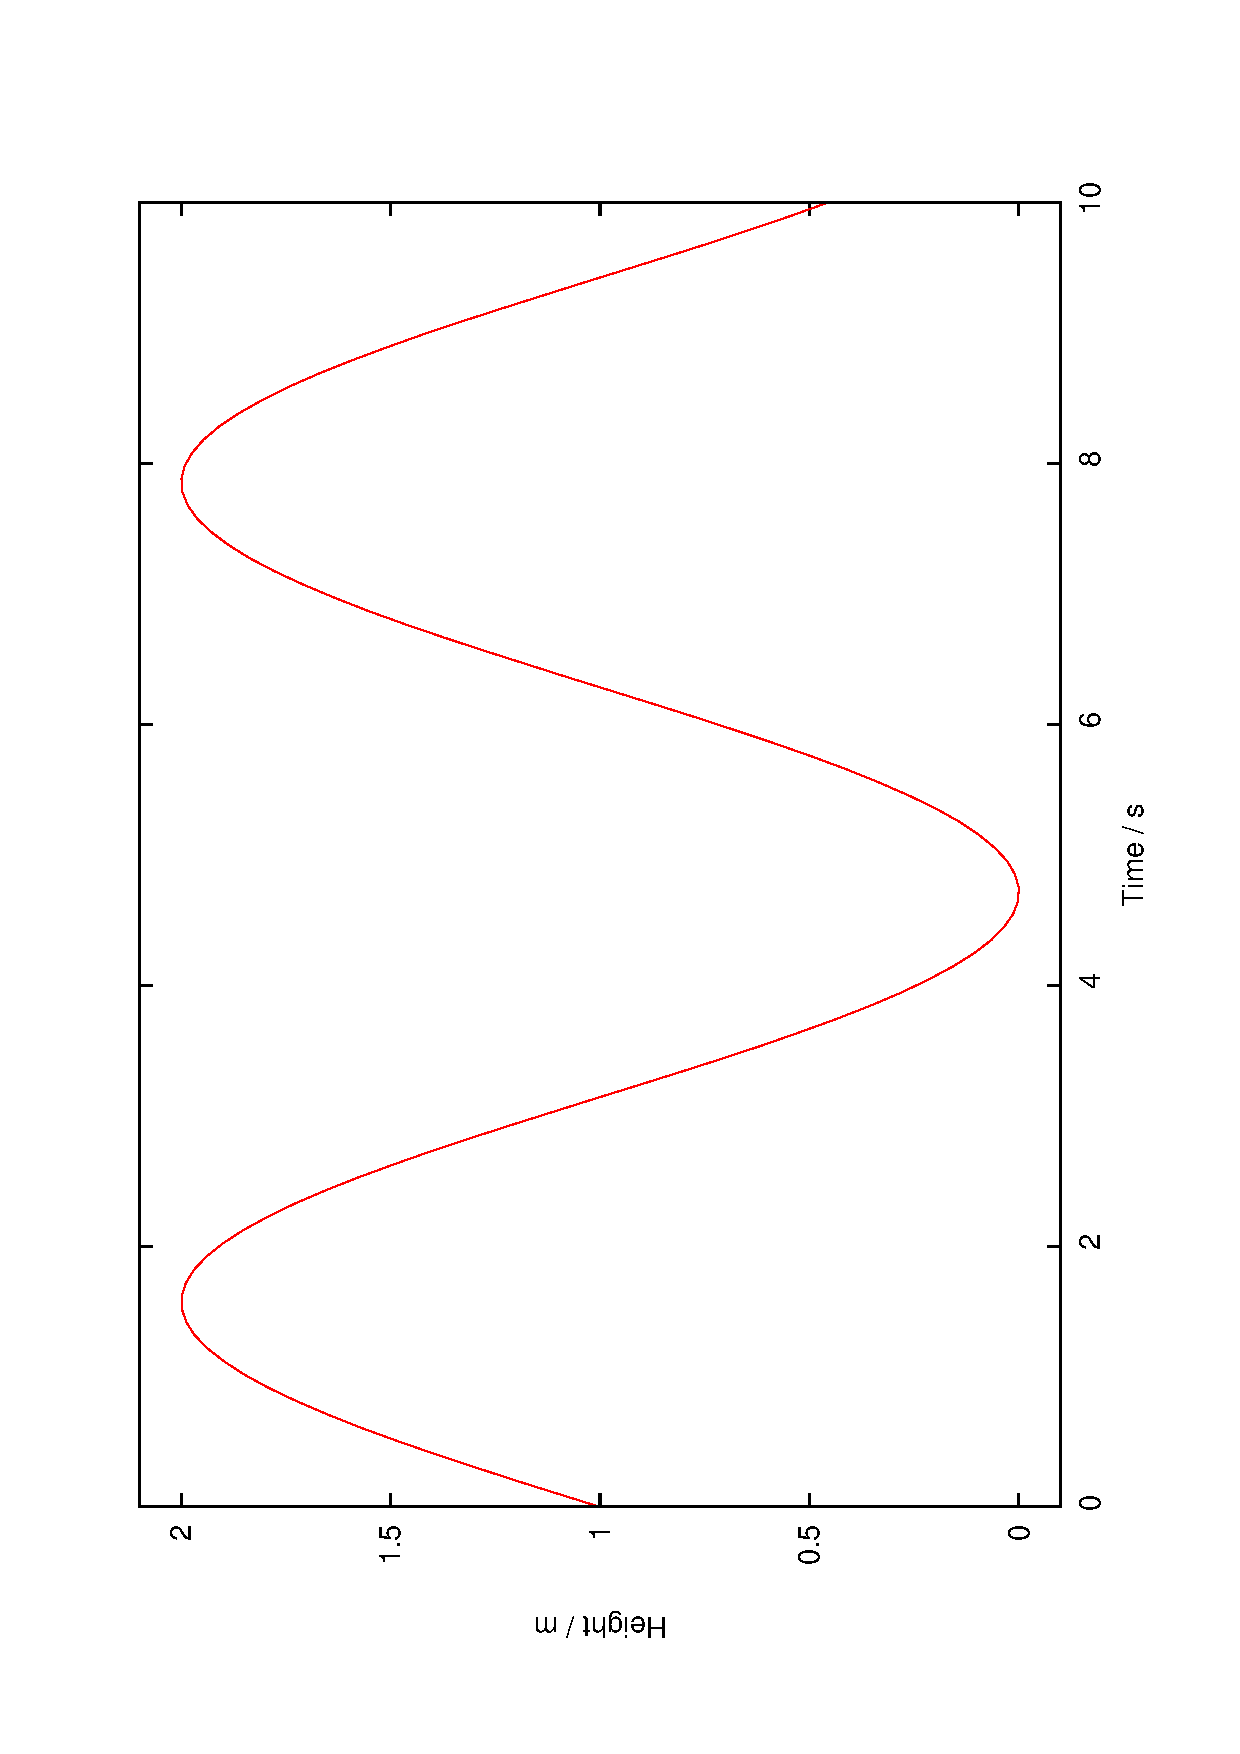
\includegraphics[width=\columnwidth]{example}
 \caption{An example figure.}
 \label{fig:example}
\end{figure}
\end{verbatim}

\begin{table}
 \caption{An example table.}
 \label{tab:example}
 \begin{tabular}{lcc}
  \hline
  Star & Mass & Luminosity\\
   & $M_{\sun}$ & $L_{\sun}$\\
  \hline
  Sun & 1.00 & 1.00\\
  $\alpha$~Cen~A & 1.10 & 1.52\\
  $\epsilon$~Eri & 0.82 & 0.34\\
  \hline
 \end{tabular}
\end{table}
The example Table~\ref{tab:example} was generated using the code:
\begin{verbatim}
\begin{table}
 \caption{An example table.}
 \label{tab:example}
 \begin{tabular}{lcc}
  \hline
  Star & Mass & Luminosity\\
   & $M_{\sun}$ & $L_{\sun}$\\
  \hline
  Sun & 1.00 & 1.00\\
  $\alpha$~Cen~A & 1.10 & 1.52\\
  $\epsilon$~Eri & 0.82 & 0.34\\
  \hline
 \end{tabular}
\end{table}
\end{verbatim}

\subsection{Captions and placement}
Captions go \emph{above} tables but \emph{below} figures, as in the examples above.

The \LaTeX\ float placement commands \verb'[htbp]' are intentionally disabled.
Layout of figures and tables will be adjusted by the publisher during the production process, so authors should not concern themselves with placement to avoid disappointment and wasted effort.
Simply place the \LaTeX\ code close to where the figure or table is first mentioned in the text and leave exact placement to the publishers.

By default a figure or table will occupy one column of the page.
To produce a wider version which covers both columns, use the \verb'figure*' or \verb'table*'  environment.

If a figure or table is too long to fit on a single page it can be split it into several parts.
Create an additional figure or table which uses \verb'\contcaption{}' instead of \verb'\caption{}'.
This will automatically correct the numbering and add `\emph{continued}' at the start of the caption.
\begin{table}
 \contcaption{A table continued from the previous one.}
 \label{tab:continued}
 \begin{tabular}{lcc}
  \hline
  Star & Mass & Luminosity\\
   & $M_{\sun}$ & $L_{\sun}$\\
  \hline
  $\tau$~Cet & 0.78 & 0.52\\
  $\delta$~Pav & 0.99 & 1.22\\
  $\sigma$~Dra & 0.87 & 0.43\\
  \hline
 \end{tabular}
\end{table}
Table~\ref{tab:continued} was generated using the code:

\begin{verbatim}
\begin{table}
 \contcaption{A table continued from the previous one.}
 \label{tab:continued}
 \begin{tabular}{lcc}
  \hline
  Star & Mass & Luminosity\\
   & $M_{\sun}$ & $L_{\sun}$\\
  \hline
  $\tau$~Cet & 0.78 & 0.52\\
  $\delta$~Pav & 0.99 & 1.22\\
  $\sigma$~Dra & 0.87 & 0.43\\
  \hline
 \end{tabular}
\end{table}
\end{verbatim}

To produce a landscape figure or table, use the \verb'pdflscape' package and the \verb'landscape' environment.
The landscape Table~\ref{tab:landscape} was produced using the code:
\begin{verbatim}
\begin{landscape}
 \begin{table}
  \caption{An example landscape table.}
  \label{tab:landscape}
  \begin{tabular}{cccccccccc}
    \hline
    Header & Header & ...\\
    Unit & Unit & ...\\
    \hline
    Data & Data & ...\\
    Data & Data & ...\\
    ...\\
    \hline
  \end{tabular}
 \end{table}
\end{landscape}
\end{verbatim}
Unfortunately this method will force a page break before the table appears.
More complicated solutions are possible, but authors shouldn't worry about this.

\begin{landscape}
 \begin{table}
  \caption{An example landscape table.}
  \label{tab:landscape}
  \begin{tabular}{cccccccccc}
    \hline
    Header & Header & Header & Header & Header & Header & Header & Header & Header & Header\\
    Unit & Unit & Unit & Unit & Unit & Unit & Unit & Unit & Unit & Unit \\
    \hline
    Data & Data & Data & Data & Data & Data & Data & Data & Data & Data\\
    Data & Data & Data & Data & Data & Data & Data & Data & Data & Data\\
    Data & Data & Data & Data & Data & Data & Data & Data & Data & Data\\
    Data & Data & Data & Data & Data & Data & Data & Data & Data & Data\\
    Data & Data & Data & Data & Data & Data & Data & Data & Data & Data\\
    Data & Data & Data & Data & Data & Data & Data & Data & Data & Data\\
    Data & Data & Data & Data & Data & Data & Data & Data & Data & Data\\
    Data & Data & Data & Data & Data & Data & Data & Data & Data & Data\\
    \hline
  \end{tabular}
 \end{table}
\end{landscape}

\section{References and citations}

\subsection{Cross-referencing}

The usual \LaTeX\ commands \verb'\label{}' and \verb'\ref{}' can be used for cross-referencing within the same paper.
We recommend that you use these whenever relevant, rather than writing out the section or figure numbers explicitly.
This ensures that cross-references are updated whenever the numbering changes (e.g. during revision) and provides clickable links (if available in your compiler).

It is best to give each section, figure and table a logical label.
For example, Table~\ref{tab:mathssymbols} has the label \verb'tab:mathssymbols', whilst section~\ref{sec:packages} has the label \verb'sec:packages'.
Add the label \emph{after} the section or caption command, as in the examples in sections~\ref{sec:sections} and \ref{sec:fig_table}.
Enter the cross-reference with a non-breaking space between the type of object and the number, like this: \verb'see Figure~\ref{fig:example}'.

The \verb'\autoref{}' command can be used to automatically fill out the type of object, saving on typing.
It also causes the link to cover the whole phrase rather than just the number, but for that reason is only suitable for single cross-references rather than ranges.
For example, \verb'\autoref{tab:journal_abbr}' produces \autoref{tab:journal_abbr}.

\subsection{Citations}
\label{sec:cite}

MNRAS uses the Harvard -- author (year) -- citation style, e.g. \citet{author2013}.
This is implemented in \LaTeX\ via the \verb'natbib' package, which in turn is included via the \verb'usenatbib' package option (see section~\ref{sec:options}), which should be used in all papers.

Each entry in the reference list has a `key' (see section~\ref{sec:ref_list}) which is used to generate citations.
There are two basic \verb'natbib' commands:
\begin{description}
 \item \verb'\citet{key}' produces an in-text citation: \citet{author2013}
 \item \verb'\citep{key}' produces a bracketed (parenthetical) citation: \citep{author2013}
\end{description}
Citations will include clickable links to the relevant entry in the reference list, if supported by your \LaTeX\ compiler.

\defcitealias{smith2014}{Paper~I}
\begin{table*}
 \caption{Common citation commands, provided by the \texttt{natbib} package.}
 \label{tab:natbib}
 \begin{tabular}{lll}
  \hline
  Command & Ouput & Note\\
  \hline
  \verb'\citet{key}' & \citet{smith2014} & \\
  \verb'\citep{key}' & \citep{smith2014} & \\
  \verb'\citep{key,key2}' & \citep{smith2014,jones2015} & Multiple papers\\
  \verb'\citet[table 4]{key}' & \citet[table 4]{smith2014} & \\
  \verb'\citep[see][figure 7]{key}' & \citep[see][figure 7]{smith2014} & \\
  \verb'\citealt{key}' & \citealt{smith2014} & For use with manual brackets\\
  \verb'\citeauthor{key}' & \citeauthor{smith2014} & If already cited in close proximity\\
  \verb'\defcitealias{key}{Paper~I}' &  & Define an alias (doesn't work in floats)\\
  \verb'\citetalias{key}' & \citetalias{smith2014} & \\
  \verb'\citepalias{key}' & \citepalias{smith2014} & \\
  \hline
 \end{tabular}
\end{table*}

There are a number of other \verb'natbib' commands which can be used for more complicated citations.
The most commonly used ones are listed in Table~\ref{tab:natbib}.
For full guidance on their use, consult the \verb'natbib' documentation\footnote{\url{http://www.ctan.org/pkg/natbib}}.

If a reference has several authors, \verb'natbib' will automatically use `et al.' if there are more than two authors. However, if a paper has exactly three authors, MNRAS style is to list all three on the first citation and use `et al.' thereafter. If you are using \bibtex\ (see section~\ref{sec:ref_list}) then this is handled automatically. If not, the \verb'\citet*{}' and \verb'\citep*{}' commands can be used at the first citation to include all of the authors.

\subsection{The list of references}
\label{sec:ref_list}

It is possible to enter references manually using the usual \LaTeX\ commands, but we strongly encourage authors to use \bibtex\ instead.
\bibtex\ ensures that the reference list is updated automatically as references are added or removed from the paper, puts them in the correct format, saves on typing, and the same reference file can be used for many different papers -- saving time hunting down reference details.
An MNRAS \bibtex\ style file, \verb'mnras.bst', is distributed as part of this package.
The rest of this section will assume you are using \bibtex.

References are entered into a separate \verb'.bib' file in standard \bibtex\ formatting.
This can be done manually, or there are several software packages which make editing the \verb'.bib' file much easier.
We particularly recommend \textsc{JabRef}\footnote{\url{http://jabref.sourceforge.net/}}, which works on all major operating systems.
\bibtex\ entries can be obtained from the NASA Astrophysics Data System\footnote{\label{foot:ads}\url{http://adsabs.harvard.edu}} (ADS) by clicking on `Bibtex entry for this abstract' on any entry.
Simply copy this into your \verb'.bib' file or into the `BibTeX source' tab in \textsc{JabRef}.

Each entry in the \verb'.bib' file must specify a unique `key' to identify the paper, the format of which is up to the author.
Simply cite it in the usual way, as described in section~\ref{sec:cite}, using the specified key.
Compile the paper as usual, but add an extra step to run the \texttt{bibtex} command.
Consult the documentation for your compiler or latex distribution.

Correct formatting of the reference list will be handled by \bibtex\ in almost all cases, provided that the correct information was entered into the \verb'.bib' file.
Note that ADS entries are not always correct, particularly for older papers and conference proceedings, so may need to be edited.
If in doubt, or if you are producing the reference list manually, see the MNRAS instructions to authors$^{\ref{foot:itas}}$ for the current guidelines on how to format the list of references.

\section{Appendices and online material}

To start an appendix, simply place the \verb'\appendix' command before the next \verb'\section{}'.
This will automatically adjust the section headings, figures, tables, and equations to reflect the fact that they are part of an appendix.
It is only necessary to enter the \verb'\appendix' command once -- everything after that command is in an appendix.
Remember that appendices should be placed \textit{after} the list of references.

Unlike other astronomy class files, there are no special commands for online material.
If your paper has any online material, it should be placed in a separate file.
See our instructions to authors$^{\ref{foot:itas}}$ for guidance.

\section{Packages and custom commands}
\label{sec:packages}
\subsection{Additional packages}

Sometimes authors need to include additional \LaTeX\ packages, which provide extra features.
For example, the \verb'bm' package provides extra bold maths symbols, whilst the \verb'pdflscape' package adds support for landscape pages.
Packages can be included by adding the \verb'\usepackage{}' command to the preamble of the document (not the main body).

Please \emph{only include packages which are actually used in the paper}, and include a comment to explain what each one does.
This will assist the typesetters.
If you are using \texttt{mnras\_template.tex}, it includes a specific section for this purpose, near the start of the file with the header 'authors - place your own packages here'.

For example, to include \verb'pdflscape', use:
\begin{verbatim}
\usepackage{pdflscape}	% Landscape pages
\end{verbatim}
Consult the documentation for that package for instructions on how to use the additional features.


\subsection{Custom commands}

Authors should avoid duplicating or redefining commands which are already available in \LaTeX\ or \verb'mnras.cls'.
However it may sometimes be necessary to introduce a custom command e.g. as a shortcut while writing the paper.

Please \emph{only include commands which are actually used in the paper}, and include a comment to explain what each one does.
This will assist the typesetters.
Use \verb'\newcommand', \emph{not} \verb'\def', as this will avoid accidentally overwriting existing commands.
Place custom commands in the preamble of the document (not the main body).
If you are using \texttt{mnras\_template.tex}, it includes a specific section for this purpose, near the start of the file with the header 'authors - place your own commands here'.

As an example, a shortcut for the unit \kms can be defined like this:
\begin{verbatim}
\newcommand{\kms}{\,km\,s$^{-1}$}	% kilometres per second
\end{verbatim}
Velocities can then be written as e.g. \verb'2.3\kms' which produces 2.3\kms.
Similar shortcuts can be used for frequently quoted object designations.


\section*{Acknowledgements}
% Entry for the table of contents, for this guide only
\addcontentsline{toc}{section}{Acknowledgements}

This guide replaces an earlier one originally prepared by Cambridge University Press (CUP) in 1994, and last updated in 2002 by Blackwell Publishing.
Some code segments are reproduced from, and some examples are based upon, that guide.
The authors were: A.~Woollatt, M.~Reed, R.~Mulvey, K.~Matthews, D.~Starling, Y.~Yu, A.~Richardson (all CUP), and Penny~Smith, N.~Thompson and Gregor~Hutton (all Blackwell), whose work is gratefully acknowledged.

The accompanying \bibtex\ style file was written by John Sleath, Tim Jenness and Norman Gray, without whom \bibtex\ support would not have been possible.

Some special symbols in tables~\ref{tab:anysymbols}--\ref{tab:mathssymbols} were taken from the Springer Verlag \textit{Astronomy \& Astrophysics} \LaTeX\ class, with their permission.

KTS thanks Nelson Beebe (University of Utah) for helpful advice regarding CTAN.

%%%%%%%%%%%%%%%%%%%%%%%%%%%%%%%%%%%%%%%%%%%%%%%%%%

%%%%%%%%%%%%%%%%%%%% REFERENCES %%%%%%%%%%%%%%%%%%

% The best way to enter references is to use BibTeX:

%\bibliographystyle{mnras}
%\bibliography{example} % if your bibtex file is called example.bib


% Alternatively you could enter them by hand, like this:
\begin{thebibliography}{99}
\bibitem[\protect\citeauthoryear{Author}{2013}]{author2013}
Author A.~N., 2013, Journal of Improbable Astronomy, 1, 1
\bibitem[\protect\citeauthoryear{Jones}{2015}]{jones2015}
Jones C.~D., 2015, Journal of Interesting Stuff, 17, 198
\bibitem[\protect\citeauthoryear{Smith}{2014}]{smith2014}
Smith A.~B., 2014, The Example Journal, 12, 345 (Paper I)
\end{thebibliography}


%%%%%%%%%%%%%%%%%%%%%%%%%%%%%%%%%%%%%%%%%%%%%%%%%%

%%%%%%%%%%%%%%%%% APPENDICES %%%%%%%%%%%%%%%%%%%%%

\appendix
\section{Journal abbreviations}
\label{sec:abbreviations}
Abbreviations for cited journals can be accessed using the commands listed in table~\ref{tab:journal_abbr}.
Although some of these may appear to be outdated or rarely cited, they have been selected to be compatible with the \bibtex\ output by the NASA Astrophysics Data System$^{\ref{foot:ads}}$, commands used by other astronomy journals, and with additional entries for journals with non-standard abbreviations in MNRAS.
For journals which are not on this list, see our instructions to authors$^{\ref{foot:itas}}$ for guidance on how to abbreviate titles.

\begin{table*}
\caption{Commands for abbreviated journal names, see appendix~\ref{sec:abbreviations}.}
\label{tab:journal_abbr}
\begin{tabular}{@{}l@{\:}l@{\:}l@{}} % manual @ spacing to prevent this being too wide for a page
\hline
Command & Output & Journal name\\
\hline
\verb'\aap' or \verb'\astap' & \aap & Astronomy and Astrophysics$^a$\\
\verb'\aapr' & \aapr & The Astronomy and Astrophysics Review\\
\verb'\aaps' & \aaps  & Astronomy and Astrophysics Supplement Series\\
\verb'\actaa' & \actaa & Acta Astronomica\\
\verb'\afz' & \afz & Astrofizika\\
\verb'\aj' & \aj & The Astronomical Journal\\
\verb'\ao' or \verb'\applopt' & \ao & Applied Optics\\
\verb'\aplett' & \aplett & Astrophysics Letters\\
\verb'\apj' & \apj & The Astrophysical Journal\\
\verb'\apjl' or \verb'\apjlett' & \apjl & The Astrophysical Journal Letters$^a$\\
\verb'\apjs' or \verb'\apjsupp' & \apjs & The Astrophysical Journal Supplement Series\\
\verb'\apss' & \apss & Astrophysics and Space Science\\
\verb'\araa' & \araa & Annual Review of Astronomy and Astrophysics\\
\verb'\arep' & \arep & Astronomy Reports$^b$\\
\verb'\aspc' & \aspc & Astronomical Society of the Pacific Conference Series\\
\verb'\azh' & \azh & Astronomicheskii Zhurnal$^c$\\
\verb'\baas' & \baas & Bulletin of the American Astronomical Society\\
\verb'\bac' & \bac & Bulletin of the Astronomical Institutes of Czechoslovakia\\
\verb'\bain' & \bain & Bull. Astron. Inst. Netherlands\\
\verb'\caa' & \caa & Chinese Astronomy and Astrophysics\\
\verb'\cjaa' & \cjaa & Chinese Journal of Astronomy and Astrophysics\\
\verb'\fcp' & \fcp & Fundamentals of Cosmic Physics\\
\verb'\gca' & \gca & Geochimica Cosmochimica Acta\\
\verb'\grl' & \grl & Geophysics Research Letters\\
\verb'\iaucirc' & \iaucirc & International Astronomical Union Circulars\\
\verb'\icarus' & \icarus & Icarus\\
\verb'\japa' & \japa & Journal of Astrophysics and Astronomy\\
\verb'\jcap' & \jcap & Journal of Cosmology and Astroparticle Physics\\
\verb'\jcp' & \jcp & Journal of Chemical Physics\\
\verb'\jgr' & \jgr & Journal of Geophysics Research\\
\verb'\jqsrt' & \jqsrt & Journal of Quantitiative Spectroscopy and Radiative Transfer\\
\verb'\jrasc' & \jrasc & Journal of the Royal Astronomical Society of Canada\\
\verb'\memras' & \memras & Memoirs of the Royal Astronomical Society\\
\verb'\memsai' & \memsai & Memoire della Societa Astronomica Italiana\\
\verb'\mnassa' & \mnassa & Monthly Notes of the Astronomical Society of Southern Africa\\
\verb'\mnras' & \mnras & Monthly Notices of the Royal Astronomical Society$^a$\\
\verb'\na' & \na & New Astronomy\\
\verb'\nar' & \nar & New Astronomy Review\\
\verb'\nat' & \nat & Nature\\
\verb'\nphysa' & \nphysa & Nuclear Physics A\\
\verb'\pra' & \pra & Physical Review A: Atomic, molecular, and optical physics\\
\verb'\prb' & \prb & Physical Review B: Condensed matter and materials physics\\
\verb'\prc' & \prc & Physical Review C: Nuclear physics\\
\verb'\prd' & \prd & Physical Review D: Particles, fields, gravitation, and cosmology\\
\verb'\pre' & \pre & Physical Review E: Statistical, nonlinear, and soft matter physics\\
\verb'\prl' & \prl & Physical Review Letters\\
\verb'\pasa' & \pasa & Publications of the Astronomical Society of Australia\\
\verb'\pasp' & \pasp & Publications of the Astronomical Society of the Pacific\\
\verb'\pasj' & \pasj & Publications of the Astronomical Society of Japan\\
\verb'\physrep' & \physrep & Physics Reports\\
\verb'\physscr' & \physscr & Physica Scripta\\
\verb'\planss' & \planss & Planetary and Space Science\\
\verb'\procspie' & \procspie & Proceedings of the Society of Photo-Optical Instrumentation Engineers\\
\verb'\rmxaa' & \rmxaa & Revista Mexicana de Astronomia y Astrofisica\\
\verb'\qjras' & \qjras & Quarterly Journal of the Royal Astronomical Society\\
\verb'\sci' & \sci & Science\\
\verb'\skytel' & \skytel & Sky and Telescope\\
\verb'\solphys' & \solphys & Solar Physics\\
\verb'\sovast' & \sovast & Soviet Astronomy$^b$\\
\verb'\ssr' & \ssr & Space Science Reviews\\
\verb'\zap' & \zap & Zeitschrift fuer Astrophysik\\
\hline
\multicolumn{3}{l}{$^a$ Letters are designated by an L at the start of the page number, not in the journal name}\\
\multicolumn{3}{l}{$^b$ In 1992 the English translation of this journal changed its name from Soviet Astronomy to Astronomy Reports}\\
\multicolumn{3}{l}{$^c$ Including the English translation Astronomy Letters}\\
\end{tabular}
\end{table*}

\clearpage % to avoid the long table breaking up the formatting examples
\section{Advanced formatting examples}
\label{sec:advanced}

Sometimes formatting doesn't behave exactly as expected when used in titles or section headings, and must be modified to obtain the correct appearance.
Generally the publishers can fix these problems during the typesetting process after a paper is accepted, but authors may wish to adjust these themselves to minimise the possibility of errors and/or for the benefit of the refereeing process.
Below are some examples of output, followed by the \LaTeX\ code which produces them.

Most mathematics and text formatting works as expected, but some commands might not be the correct size, bold or italic.
If so they can be finessed by hand, as in the bold mathematics here:
\boxit{\huge\bf \textit{Herschel} observations of galaxies at $\bm{\delta > 60\degr}$}
\begin{verbatim}
\title{\textit{Herschel} observations of galaxies at
 $\bm{\delta > 60\degr}$}
\end{verbatim}

Most fonts do not provide bold and italic versions of small capitals, so the \verb'\ion{}{}' command doesn't produce the expected output in headings.
The effect has to be `faked' using font size commands, remembering that the running head is a different style:
\boxit{\huge\bf Abundances in H\,{\Large \textbf{II}} regions}
\begin{verbatim}
\title
[Abundances in H\,{\normalsize \textit{II}} regions]
{Abundances in H\,{\Large \textbf{II}} regions}
\end{verbatim}

Complex mathematics can cause problems with links, so might require adding a less formatted short version of the heading:
\boxit{\bf 2\quad FINDING Mg\,{\sevensize II} ABSORBERS AT $\bm{z > 2}$}
\begin{verbatim}
\section
[Finding Mg II absorbers at z > 2]
{Finding M\lowercase{g}\,{\sevensize II} absorbers
 at $\lowercase{\bm{z > 2}}$}
\end{verbatim}


Using square brackets in headings can cause additional linking problems, which are solved by wrapping them in \{\textellipsis\}:
\boxit{\bf 2.1\quad [C\,{\sevensize II}] 158$\bmath{\umu}$m emission}
\begin{verbatim}
\subsection
[{[C II] 158$\umu$m emission}]
{[C\,{\sevensize II}] 158$\bmath{\umu}$m
 emission}
\end{verbatim}

Use \verb'\text{}' (not \verb'\rm') for non-variables in mathematics, which preserves the formatting of the surrounding text.
For the same reasons, use \verb'\textit{}' for italics (not \verb'\it').
\boxit{\bf 3.1\quad Measuring $\bm{T}_\text{eff}$ from \textit{Gaia} photometry}
\begin{verbatim}
\subsection{Measuring $\bm{T}_\text{eff}$ from
 \textit{Gaia} photometry}
\end{verbatim}

\section{Additional commands for editors only}
The following commands are available for the use of editors and production staff only.
They should not be used (or modified in the template) by authors.

\begin{description}
 \item \verb'\maketitle' inserts the title, authors and institution list in the correct formatting.
 \item \verb'\nokeywords' tidies up the spacing if there are no keywords, but authors should always enter at least one.
 \item \verb'\volume{}' sets the volume number (default is 000)
 \item \verb'\pagerange{}' sets the page range. The standard template generates this automatically, starting from 1.
 \item \verb'\bsp' adds the `This paper has been typeset\textellipsis' comment at the end of the paper.
The command name refers to Blackwell Science Publishing, who were the publishers at the time when MNRAS began accepting \LaTeX\ submissions in 1993.
 \item \verb'\mniiiauth{}' used by the \bibtex\ style to handle MNRAS style for citing papers with three authors. It should not be used manually.
 \item \verb'\eprint{}' used by the \bibtex\ style for citing arXiv eprints.
 \item \verb'\doi{}' used by the \bibtex\ style for citing Digital Object Identifiers.
\end{description}

%%%%%%%%%%%%%%%%%%%%%%%%%%%%%%%%%%%%%%%%%%%%%%%%%%


% Don't change these lines
\bsp	% typesetting comment
\label{lastpage}
\end{document}

% End of mnras_guide.tex